\chapter{บทนำ}

\par{
ก่อนจะถึงในรายละเอียดข้างต้น 
ในส่วนแรกจะกล่าวถึงประวัติและความเป็นมาของ
ระบบการคำนวณอันเป็นที่มาของสถาปัตยกรรมคอมพิวเตอร์
}

\par{
Charles Babbage เป็นศาสตราจารย์ในสาขาคณิตศาสตร์ที่มหาวิทยาลัย 
Cambridge ในช่วง 1827 ถึง 1839 ซึ่งถูกยกย่องว่า
เป็นบิดาแห่งคอมพิวเตอร์ (father of the computer) [1] 
เนื่องจากเป็นผู้คิดค้นเครื่องคำนวณแบบจักรกลเป็นผลสำเร็จเป็นคนแรก อันนำมาซึ่งในการออกแบบเครื่องคำนวณในรูปแบบต่าง ๆ ที่มีความซับซ้อนมากยิ่งขึ้น หนึ่งในเครื่องจักรการคำนวณที่จะกล่าวถึงคือ Different Engine (ถูกออกแบบในปี 1823) ดังแสดงในรูปที่ 1
}

\begin{figure}[h]
\caption{Different Engine ที่ถูกจัดแสดงใน London Science Museum}
\centering
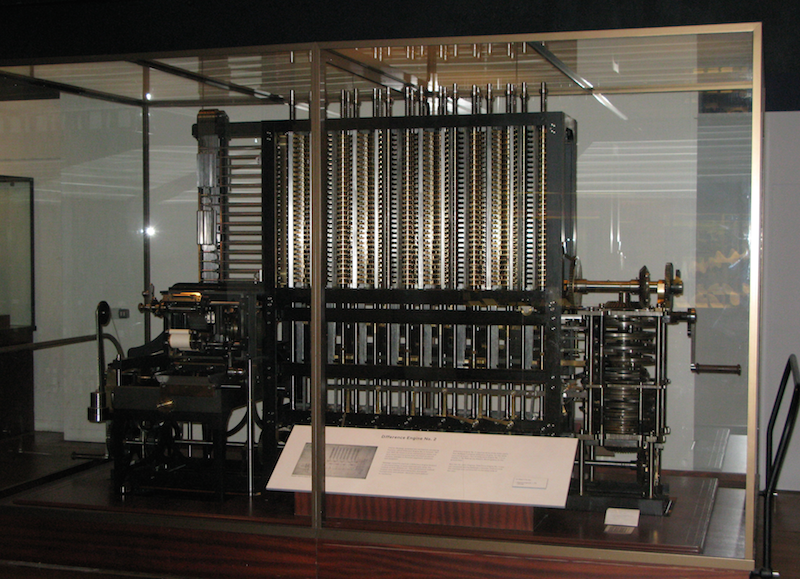
\includegraphics[width=0.75\textwidth]{fig/Babbage_Difference_Engine.png}
\end{figure}

